%%%%%%%%%%%%%%%%%%%%%%%%%%%%%%%%%%%%%%%%%%%%%%%%%%%%%%%%%%%%%%%%%%%%%%
\section{\label{sec:Configuring-Policy}
Configuring The Startd Policy}
%%%%%%%%%%%%%%%%%%%%%%%%%%%%%%%%%%%%%%%%%%%%%%%%%%%%%%%%%%%%%%%%%%%%%%

This section describes how to configure the \Condor{startd} to
implement the policy you choose for when remote jobs should start, be
suspended, (possibly) resumed, vacated (with a checkpoint) or killed
(no checkpoint).  This policy is the heart of Condor's balancing act
between the needs and wishes of resource owners (machine owners) and
resource users (people submitting their jobs to Condor).  Please read
this section carefully if you plan to change any of the settings
described below, as getting it wrong can have a severe impact on
either the owners of machines in your pool (in which case they might
ask to be removed from the pool entirely) or the users of your pool
(in which case they might stop using Condor).

Much of this section refers to ClassAd expressions.  You probably want
to read through section~\ref{classad-reference} on ClassAd expressions
before continuing with this.

\Note If you are defining the policy for an SMP (multi-CPU) machine,
be sure to also read section~\ref{sec:Configuring-SMP} on
``Configuring The Startd for SMP Machines''.  
Each \Term{virtual machine} represented by the \condor{startd} on an
SMP machine will have its own \Term{state} and \Term{activity}
(described below). 
In the future, each virtual machine will even be able to have its
own policy defined.
For the rest of this section, whenever you see the word ``machine'',
that really just means an individual virtual machine, if you're
talking about an SMP machine that is showing up as multiple virtual
machines in your pool.  

To define your policy, you basically set a number of expressions in
the config file (see section~\ref{sec:Configuring-Condor} on
``Configuring Condor'' for an introduction to Condor's config files).
These expressions are evaluated in the context of the machine's ClassAd
and the ClassAd of a potential resource request (a job that has been
submitted to Condor).
The expressions can therefore reference attributes from either
ClassAd. 
First, we'll list all the attributes that are included in the Machine's
ClassAd.
Then, we'll list all the attributes that are included in a job
ClassAd. 
Next, we'll explain the the \Expr{START} expression, which describes
to Condor what conditions must be met for the machine to start a job.
Then, we'll describe the \Expr{RANK} expression, which allows you to
specify which kinds of jobs a given machine prefers to run.
Then, we'll discuss in some detail how the \Condor{startd} works, in
particular, the machine \Term{states} and \Term{activities}, to give
you an idea of what is possible for your policy decisions.
Finally, we offer two example policy settings.

%%%%%%%%%%%%%%%%%%%%%%%%%%%%%%%%%%%%%%%%%%%%%%%%%%%%%%%%%%%%%%%%%%%%%%
\subsection{\label{sec:Startd-Attributes}
Startd ClassAd Attributes}
%%%%%%%%%%%%%%%%%%%%%%%%%%%%%%%%%%%%%%%%%%%%%%%%%%%%%%%%%%%%%%%%%%%%%%

The \Condor{startd} represents the machine on which it is running to
the Condor pool.  It publishes a number of characteristics about the
machine in its ClassAd to help in match-making with resource requests.
The values of all these attributes can be found by using
\Prog{\condor{status} -l hostname}.
On an SMP machine, the startd will break the machine up and advertise
it as seperate virtual machines, each with its own name and ClassAd.
The attributes themselves and what they represent are described below:

\begin{description}
%
\index{ClassAd!machine attributes}
\index{ClassAd machine attribute!Activity}
\item[\AdAttr{Activity}:] String which describes HTCondor job activity on the machine.
Can have one of the following values:
	\begin{description}
	\item[\AdStr{Idle}:] There is no job activity
	\item[\AdStr{Busy}:] A job is busy running
	\item[\AdStr{Suspended}:] A job is currently suspended
	\item[\AdStr{Vacating}:] A job is currently checkpointing
	\item[\AdStr{Killing}:] A job is currently being killed
	\item[\AdStr{Benchmarking}:] The startd is running benchmarks
	\item[\AdStr{Retiring}:] Waiting for a job to finish or for the maximum retirement time to expire
	\end{description}
%
\index{ClassAd machine attribute!Arch}
\label{Arch-machine-attribute}
\item[\AdAttr{Arch}:] String with the architecture of the machine.  
Currently supported architectures have the following string
definitions:
	\begin{description}
	\item[\AdStr{INTEL}:] Intel x86 CPU (Pentium, Xeon, etc).
	\item[\AdStr{X86\_64}:] AMD/Intel 64-bit X86
	\end{description}
These strings show definitions for architectures no longer supported:
	\begin{description}
	\item[\AdStr{IA64}:] Intel Itanium
	\item[\AdStr{SUN4u}:] Sun UltraSparc CPU
	\item[\AdStr{SUN4x}:] A Sun Sparc CPU other than an UltraSparc, i.e.
sun4m or sun4c CPU found in older Sparc workstations such as the Sparc~10, 
Sparc~20, IPC, IPX, etc.
	\item[\AdStr{PPC}:] 32-bit PowerPC
	\item[\AdStr{PPC64}:] 64-bit PowerPC
	\end{description}
%
\index{ClassAd machine attribute!CanHibernate}
\item[\AdAttr{CanHibernate}:] The \Condor{startd} has the capability to 
shut down or hibernate a machine when certain configurable criteria are met.
However, before the \Condor{startd} can shut down a machine, 
the hardware itself must support hibernation, as must the operating system. 
When the \Condor{startd} initializes, 
it checks for this support.
If the machine has the ability to hibernate, 
then this boolean ClassAd attribute will be \Expr{True}.
By default, it is \Expr{False}.
%
\index{ClassAd machine attribute!CheckpointPlatform}
\label{CheckpointPlatform-machine-attribute}
\item[\AdAttr{CheckpointPlatform}:] A string which opaquely encodes various
aspects about a machine's operating system, hardware, and kernel
attributes.
It is used to identify systems where previously taken checkpoints for
the standard universe may resume.
%
\index{ClassAd machine attribute!ClockDay}
\item[\AdAttr{ClockDay}:] The day of the week, 
where 0 = Sunday, 1 = Monday, \Dots, and 6 = Saturday. 
%
\index{ClassAd machine attribute!ClockMin}
\item[\AdAttr{ClockMin}:] The number of minutes passed since midnight.
%
\index{ClassAd machine attribute!CondorLoadAvg}
\item[\AdAttr{CondorLoadAvg}:] The load average contributed  
by HTCondor, either from remote jobs or running benchmarks.
%
\index{ClassAd machine attribute!CondorVersion}
\item[\AdAttr{CondorVersion}:] A string containing the HTCondor version
number for the \Condor{startd} daemon, the release date, and the build
identification number.
%
\index{ClassAd machine attribute!ConsoleIdle}
\item[\AdAttr{ConsoleIdle}:] The number of seconds since activity on the system
console keyboard or console mouse has last been detected.
The value can be modified with \Macro{SLOTS\_CONNECTED\_TO\_CONSOLE}
as defined at ~\ref{param:SlotsConnectedToConsole}.
%
\index{ClassAd machine attribute!Cpus}
\item[\AdAttr{Cpus}:]  The number of CPUs in this slot.
It is 1 for a single CPU slot, 2 for a dual CPU slot, etc.
%
\index{ClassAd machine attribute!CurrentRank}
\item[\AdAttr{CurrentRank}:] A float which represents this machine
owner's affinity
for running the HTCondor job which it is currently hosting.  If not
currently hosting an HTCondor job, \AdAttr{CurrentRank} is 0.0.
When a machine is claimed,
the attribute's value is computed by evaluating the machine's
\AdAttr{Rank} expression with respect to the current job's ClassAd.
%
\index{ClassAd machine attribute!Disk}
\item[\AdAttr{Disk}:] The amount of disk space on this machine available for
the job in Kbytes ( e.g. 23000 = 23 megabytes ).  Specifically, this
is the amount of disk space available in the directory specified in
the HTCondor configuration files by the \Macro{EXECUTE} macro, minus any
space reserved with the \Macro{RESERVED\_DISK} macro.
%
\index{ClassAd machine attribute!Draining}
\item[\AdAttr{Draining}:] This attribute is \Expr{True} when the slot
is draining and undefined if not.
%
\index{ClassAd machine attribute!DrainingRequestId}
\item[\AdAttr{DrainingRequestId}:] This attribute contains a string that
is the request id of the draining request that put this slot in a draining
state.  It is undefined if the slot is not draining.
%
\index{ClassAd machine attribute!DotNetVersions}
\item[\AdAttr{DotNetVersions}:] The .NET framework versions
currently installed on this computer. 
Default format is a comma delimited list. 
Current definitions:
  \begin{description}
  \item[\AdStr{1.1}:] for .Net Framework 1.1
  \item[\AdStr{2.0}:] for .Net Framework 2.0
  \item[\AdStr{3.0}:] for .Net Framework 3.0
  \item[\AdStr{3.5}:] for .Net Framework 3.5
  \item[\AdStr{4.0Client}:] for .Net Framework 4.0 Client install
  \item[\AdStr{4.0Full}:] for .Net Framework 4.0 Full install
  \end{description}
%
\index{ClassAd machine attribute!DynamicSlot}
\label{DynamicSlot-machine-attribute} 
\item[\AdAttr{DynamicSlot}:] For SMP machines that allow dynamic
partitioning of a slot,
this boolean value identifies that this dynamic slot may be partitioned.
%
\index{ClassAd machine attribute!EnteredCurrentActivity}
\item[\AdAttr{EnteredCurrentActivity}:] Time at which the machine
entered the current Activity (see \AdAttr{Activity} entry above).  On
all platforms (including NT), this is measured in the number of
integer seconds since the Unix epoch (00:00:00 UTC, Jan 1, 1970).
%
\index{ClassAd machine attribute!ExpectedMachineGracefulDrainingBadput}
\item[\AdAttr{ExpectedMachineGracefulDrainingBadput}:] The
job runtime in cpu-seconds that would be lost if graceful draining
were initiated at the time this ad was published.  This calculation assumes
that jobs will run for the full retirement time and then be evicted
without saving a checkpoint.
%
\index{ClassAd machine attribute!ExpectedMachineGracefulDrainingCompletion}
\item[\AdAttr{ExpectedMachineGracefulDrainingCompletion}:] Time at
which graceful draining of the machine could complete if it were
initiated at the time this ad was published.  This is measured in the
number of integer seconds since the Unix epoch (00:00:00 UTC, Jan 1,
1970).  This value is computed with the assumption that the machine
policy will not suspend jobs during draining while the machine is
waiting for the job to use up its retirement time.  If suspension
happens, the upper bound on how long draining could take is
unlimited.  To avoid suspension during draining, the \MacroNI{SUSPEND}
and \MacroNI{CONTINUE} expressions could be configured to pay
attention to the \AdAttr{Draining} attribute.
%
\index{ClassAd machine attribute!ExpectedMachineQuickDrainingBadput}
\item[\AdAttr{ExpectedMachineGracefulQuickBadput}:] The
job runtime in cpu-seconds that would be lost if quick draining
were initiated at the time this ad was published.  This calculation assumes
that all evicted jobs will not save a checkpoint.
%
\index{ClassAd machine attribute!ExpectedMachineQuickDrainingCompletion}
\item[\AdAttr{ExpectedMachineQuickDrainingCompletion}:] Time at
which quick draining of the machine could complete if it were
initiated at the time this ad was published.  This is measured in the
number of integer seconds since the Unix epoch (00:00:00 UTC, Jan 1,
1970).
%
\index{ClassAd machine attribute!FileSystemDomain}
\item[\AdAttr{FileSystemDomain}:] A domain name configured by the
HTCondor administrator which describes a cluster of machines which all
access the same, uniformly-mounted, networked file systems usually via
NFS or AFS.  This is useful for Vanilla universe jobs which require
remote file access.
%
\index{ClassAd machine attribute!Has\_sse4\_1}
\item[\AdAttr{Has\_sse4\_1}:] A boolean value set to \Expr{True}
 if the machine being advertised supports
the SSE 4.1 instructions, and \Expr{Undefined} otherwise.
%
\index{ClassAd machine attribute!Has\_sse4\_2}
\item[\AdAttr{Has\_sse4\_2}:] A boolean value set to \Expr{True}
if the machine being advertised supports
the SSE 4.2 instructions, and \Expr{Undefined} otherwise.
%
\index{ClassAd machine attribute!has\_ssse3}
\item[\AdAttr{has\_ssse3}:] A boolean value set to \Expr{True}
if the machine being advertised supports
the SSSE 3 instructions, and \Expr{Undefined} otherwise.
%
\index{ClassAd machine attribute!HasVM}
\item[\AdAttr{HasVM}:] A boolean value added to the machine ClassAd
when the configuration triggers the detection of virtual machine
software.
%
\index{ClassAd machine attribute!IsWakeAble}
\item[\AdAttr{IsWakeAble}:] A boolean value that when \Expr{True} identifies
that the machine has the capability to be woken into a 
fully powered and running state by receiving a Wake On LAN (WOL) packet.
This ability is a function of the operating system, 
the network adapter in the machine 
(notably, wireless network adapters usually do not have this function),
and BIOS settings. 
When the \Condor{startd} initializes, 
it tries to detect if the operating system and network adapter both support 
waking from hibernation by receipt of a WOL packet.
The default value is \Expr{False}.
%
\index{ClassAd machine attribute!IsWakeEnabled}
\item[\AdAttr{IsWakeEnabled}:] If the hardware and software have the capacity 
to be woken into a fully powered and running state by receiving 
a Wake On LAN (WOL) packet,
this feature can still be disabled via the BIOS or software.
If BIOS or the operating system have disabled this feature, 
the \Condor{startd} sets this boolean attribute to \Expr{False}.
%
\index{ClassAd machine attribute!JobVM\_VCPUS}
\item[\AdAttr{JobVM\_VCPUS}:] An attribute defined if a vm universe job
is running on this slot.  Defined by the number of virtualized CPUs
in the virtual machine.
%
\index{ClassAd machine attribute!KeyboardIdle}
\item[\AdAttr{KeyboardIdle}:] The number of seconds since activity on any
keyboard or mouse associated with this machine has last been detected.
Unlike \AdAttr{ConsoleIdle}, \AdAttr{KeyboardIdle} also takes activity 
on pseudo-terminals into
account.
Pseudo-terminals have virtual keyboard activity from telnet and rlogin
sessions.  Note that \AdAttr{KeyboardIdle} will always be equal to or
less than \AdAttr{ConsoleIdle}.
The value can be modified with \Macro{SLOTS\_CONNECTED\_TO\_KEYBOARD}
as defined at ~\ref{param:SlotsConnectedToKeyboard}.
%
\index{ClassAd machine attribute!KFlops}
\item[\AdAttr{KFlops}:] Relative floating point performance as determined via a
Linpack benchmark.
%
\index{ClassAd machine attribute!LastDrainStartTime}
\item[\AdAttr{LastDrainStartTime}:] Time when draining of this
\Condor{startd} was last initiated (e.g. due to \Condor{defrag} or
\Condor{drain}).
%
\index{ClassAd machine attribute!LastHeardFrom}
\item[\AdAttr{LastHeardFrom}:] Time when the HTCondor central manager last
received a status update from this machine.  
Expressed as 
the number of integer seconds since the Unix epoch (00:00:00 UTC, Jan 1, 1970).
Note: This attribute is only inserted by the central manager once it
receives the ClassAd.
It is not present in the \Condor{startd} copy of the ClassAd.
Therefore, you could not use this attribute in defining \Condor{startd}
expressions (and you would not want to).
%
\index{ClassAd machine attribute!LoadAvg}
\item[\AdAttr{LoadAvg}:] A floating point number representing the 
current load average.
%
\index{ClassAd machine attribute!Machine}
\item[\AdAttr{Machine}:] A string with the machine's fully qualified host name.
%
\index{ClassAd machine attribute!MachineMaxVacateTime}
\item[\AdAttr{MachineMaxVacateTime}:] An integer expression that specifies
the time in seconds the machine will allow the job to gracefully shut
down.
%
\index{ClassAd machine attribute!Memory}
\item[\AdAttr{Memory}:] The amount of RAM in megabytes.
%
\index{ClassAd machine attribute!Mips}
\item[\AdAttr{Mips}:] Relative integer performance as determined via a Dhrystone
benchmark.

\index{ClassAd machine attribute!MonitorSelfAge}
\item[\AdAttr{MonitorSelfAge}:] The number of seconds that this daemon
  has been running.

\index{ClassAd machine attribute!MonitorSelfCPUUsage}
\item[\AdAttr{MonitorSelfCPUUsage}:] The fraction of recent CPU time utilized
  by this daemon. 

\index{ClassAd machine attribute!MonitorSelfImageSize}
\item[\AdAttr{MonitorSelfImageSize}:] The amount of virtual memory consumed by
  this daemon in Kbytes.

\index{ClassAd machine attribute!MonitorSelfRegisteredSocketCount}
\item[\AdAttr{MonitorSelfRegisteredSocketCount}:] The current number of sockets
  registered by this daemon.

\index{ClassAd machine attribute!MonitorSelfResidentSetSize}
\item[\AdAttr{MonitorSelfResidentSetSize}:] The amount of resident memory
  used by this daemon in Kbytes.

\index{ClassAd machine attribute!MonitorSelfSecuritySessions}
\item[\AdAttr{MonitorSelfSecuritySessions}:] The number of open (cached)
  security sessions for this daemon.

\index{ClassAd machine attribute!MonitorSelfTime}
\item[\AdAttr{MonitorSelfTime}:] The  time, represented as the number of
  second elapsed since the Unix epoch (00:00:00 UTC, Jan 1, 1970),
  at which this daemon last checked and set the attributes with names that
  begin with the string \Attr{MonitorSelf}.
  
\index{ClassAd machine attribute!MyAddress}
\item[\AdAttr{MyAddress}:] String with the IP and port address of the
\Condor{startd} daemon which is publishing this machine ClassAd.
When using CCB, \Condor{shared\_port}, and/or an additional private
network interface, that information will be included here as well.

\index{ClassAd machine attribute!MyType}
\item[\AdAttr{MyType}:] The ClassAd type; always set to the literal string \AdStr{Machine}.
%
\index{ClassAd machine attribute!Name}
\item[\AdAttr{Name}:] The name of this resource; typically the same value as
the \AdAttr{Machine} attribute, but could be customized by the site
administrator.
On SMP machines, the \Condor{startd} will divide the CPUs up into separate
slots, each with with a unique name.
These names will be of the form ``slot\#@full.hostname'', for example,
``slot1@vulture.cs.wisc.edu'', which signifies slot number 1 from
vulture.cs.wisc.edu.
%
\index{ClassAd machine attribute!OpSys}
\label{OpSys-machine-attribute}
\item[\AdAttr{OpSys}:] String describing the operating system running on this
machine.  
Currently supported operating systems have the following string
definitions:
	\begin{description}
	\item[\AdStr{LINUX}:] for LINUX 2.0.x, LINUX 2.2.x,
	LINUX 2.4.x, LINUX 2.6.x, or LINUX 3.10.0 kernel systems, as well as Scientific Linux 
        and Ubuntu 12.04
	\item[\AdStr{OSX}:] for Darwin
	\item[\AdStr{FREEBSD7}:] for FreeBSD 7
	\item[\AdStr{FREEBSD8}:] for FreeBSD 8
	\item[\AdStr{WINDOWS}:] for all versions of Windows
	\item[\AdStr{SOLARIS5.10}:] for Solaris 2.10 or 5.10
	\item[\AdStr{SOLARIS5.11}:] for Solaris 2.11 or 5.11
	\end{description}
These strings show definitions for operating systems no longer supported:
	\begin{description}
	\item[\AdStr{SOLARIS28}:] for Solaris 2.8 or 5.8
	\item[\AdStr{SOLARIS29}:] for Solaris 2.9 or 5.9
	\end{description}
%
\index{ClassAd machine attribute!OpSysAndVer}
\item[\AdAttr{OpSysAndVer}:] A string indicating an operating system and
a version number.

For Linux operating systems, it is the value of the \Attr{OpSysName} attribute 
concatenated with the string version of the \Attr{OpSysMajorVersion} attribute:
	\begin{description}
	\item[\AdStr{RedHat5}:] for RedHat Linux version 5
	\item[\AdStr{RedHat6}:] for RedHat Linux version 6
	\item[\AdStr{RedHat7}:] for RedHat Linux version 7 \emph{Beta}
	\item[\AdStr{Fedora16}:] for Fedora Linux version 16
	\item[\AdStr{Debian5}:] for Debian Linux version 5
	\item[\AdStr{Debian6}:] for Debian Linux version 6
	\item[\AdStr{Ubuntu12}:] for Ubuntu 12.04
	\item[\AdStr{SL5}:] for Scientific Linux version 5
	\item[\AdStr{SL6}:] for Scientific Linux version 6
	\item[\AdStr{SLFermi5}:] for Fermi's Scientific Linux version 5
	\item[\AdStr{SLFermi6}:] for Fermi's Scientific Linux version 6
	\item[\AdStr{SLCern5}:] for CERN's Scientific Linux version 5
	\item[\AdStr{SLCern6}:] for CERN's Scientific Linux version 6
	\end{description}
For MacOS operating systems, it is the value of the \Attr{OpSysShortName} 
attribute concatenated with the string version of the \Attr{OpSysVer} attribute: 
	\begin{description}
	\item[\AdStr{MacOSX605}:] for MacOS version 10.6.5 (Snow Leopard)
	\item[\AdStr{MacOSX703}:] for MacOS version 10.7.3 (Lion)
	\end{description}
For BSD operating systems, it is the value of the \Attr{OpSysName} attribute 
concatenated with the string version of the \Attr{OpSysMajorVersion} attribute:
	\begin{description}
	\item[\AdStr{FREEBSD7}:] for FreeBSD version 7
	\item[\AdStr{FREEBSD8}:] for FreeBSD version 8
	\end{description}
For Solaris Unix operating systems, 
it is the same value as the \Attr{OpSys} attribute: 
	\begin{description}
	\item[\AdStr{SOLARIS5.10}:] for Solaris 2.10 or 5.10
	\item[\AdStr{SOLARIS5.11}:] for Solaris 2.11 or 5.11
	\end{description}
For Windows operating systems, it is the value of the \Attr{OpSys} attribute 
concatenated with the string version of the \Attr{OpSysMajorVersion} attribute:
	\begin{description}
	\item[\AdStr{WINDOWS500}:] for Windows 2000
	\item[\AdStr{WINDOWS501}:] for Windows XP
	\item[\AdStr{WINDOWS502}:] for Windows Server 2003
	\item[\AdStr{WINDOWS600}:] for Windows Vista
	\item[\AdStr{WINDOWS601}:] for Windows 7
	\end{description}
%
\index{ClassAd machine attribute!OpSysLegacy}
\item[\AdAttr{OpSysLegacy}:] A string that holds the long-standing values for the \Attr{OpSys} attribute.
Currently supported operating systems have the following string
definitions:
	\begin{description}
	\item[\AdStr{LINUX}:] for LINUX 2.0.x, LINUX 2.2.x, LINUX 2.4.x, LINUX 2.6.x, or LINUX 3.10.0 kernel systems, as well as Scientific Linux and  Ubuntu 12.04 versions
	\item[\AdStr{OSX}:] for Darwin
	\item[\AdStr{FREEBSD7}:] for FreeBSD version 7
	\item[\AdStr{FREEBSD8}:] for FreeBSD version 8
	\item[\AdStr{SOLARIS5.10}:] for Solaris 2.10 or 5.10
	\item[\AdStr{SOLARIS5.11}:] for Solaris 2.11 or 5.11
	\item[\AdStr{WINDOWS}:] for all versions of Windows
	\end{description}
%
\index{ClassAd machine attribute!OpSysLongName}
\item[\AdAttr{OpSysLongName}:] A string giving a full description of 
the operating system.
For Linux platforms, this is generally the string taken from \File{/etc/hosts},
with extra characters stripped off Debian versions.
	\begin{description}
	\item[\AdStr{Red Hat Enterprise Linux Server release 5.7 (Tikanga)}:] for RedHat Linux version 5
	\item[\AdStr{Red Hat Enterprise Linux Server release 6.2 (Santiago)}:] for RedHat Linux version 6
	\item[\AdStr{Red Hat Enterprise Linux Everything release 7.0 (Maipo)}:] for RedHat Linux version 7.0 \emph{Beta}
	\item[\AdStr{Ubuntu 12.04.3 LTS}:] for Ubuntu 12.04 point release 3 
	\item[\AdStr{Fedora release 16 (Verne)}:] for Fedora Linux version 16
	\item[\AdStr{MacOSX 6.5}:] for MacOS version 10.6.5 (Snow Leopard)
	\item[\AdStr{MacOSX 7.3}:] for MacOS version 10.7.3 (Lion)
	\item[\AdStr{FreeBSD8.2-RELEASE-p3}:] for FreeBSD version 8
	\item[\AdStr{SOLARIS5.10}:] for Solaris 2.10 or 5.10
	\item[\AdStr{SOLARIS5.11}:] for Solaris 2.11 or 5.11
	\item[\AdStr{Windows XP SP3}:] for Windows XP
	\item[\AdStr{Windows 7 SP2}:] for Windows 7
	\end{description}
%
\index{ClassAd machine attribute!OpSysMajorVersion}
\item[\AdAttr{OpSysMajorVersion}:] An integer value representing the major version of the operating system.
	\begin{description}
	\item[\Expr{5}:] for RedHat Linux version 5 
and derived platforms such as Scientific Linux
	\item[\Expr{6}:] for RedHat Linux version 6
and derived platforms such as Scientific Linux
	\item[\Expr{7}:] for RedHat Linux version 7 \emph{Beta}
	\item[\Expr{12}:] for Ubuntu 12.04
	\item[\Expr{16}:] for Fedora Linux version 16
	\item[\Expr{6}:] for MacOS version 10.6.5 (Snow Leopard)
	\item[\Expr{7}:] for MacOS version 10.7.3 (Lion)
	\item[\Expr{7}:] for FreeBSD version 7
	\item[\Expr{8}:] for FreeBSD version 8
	\item[\Expr{5}:] for Solaris 2.10, 5.10, 2.11, or 5.11
	\item[\Expr{501}:] for Windows XP
	\item[\Expr{600}:] for Windows Vista
	\item[\Expr{601}:] for Windows 7
	\end{description}
%
\index{ClassAd machine attribute!OpSysName}
\item[\AdAttr{OpSysName}:] A string containing a terse description of the operating system.
	\begin{description}
	\item[\AdStr{RedHat}:] for RedHat Linux version 6 and 7 \emph{Beta}
	\item[\AdStr{Fedora}:] for Fedora Linux version 16
	\item[\AdStr{Ubuntu}:] for Ubuntu 12.04
	\item[\AdStr{SnowLeopard}:] for MacOS version 10.6.5 (Snow Leopard)
	\item[\AdStr{Lion}:] for MacOS version 10.7.3 (Lion)
	\item[\AdStr{FREEBSD}:] for FreeBSD version 7 or 8
	\item[\AdStr{SOLARIS5.10}:] for Solaris 2.10 or 5.10
	\item[\AdStr{SOLARIS5.11}:] for Solaris 2.11 or 5.11
	\item[\AdStr{WindowsXP}:] for Windows XP
	\item[\AdStr{WindowsVista}:] for Windows Vista
	\item[\AdStr{Windows7}:] for Windows 7
	\item[\AdStr{SL}:] for Scientific Linux
	\item[\AdStr{SLFermi}:] for Fermi's Scientific Linux
	\item[\AdStr{SLCern}:] for CERN's Scientific Linux
	\end{description}
%
\index{ClassAd machine attribute!OpSysShortName}
\item[\AdAttr{OpSysShortName}:] A string containing a short name for
the operating system.
	\begin{description}
	\item[\AdStr{RedHat}:] for RedHat Linux version 5, 6 or 7 \emph{Beta}
	\item[\AdStr{Fedora}:] for Fedora Linux version 16
	\item[\AdStr{Debian}:] for Debian Linux version 5 or 6
	\item[\AdStr{Ubuntu}:] for Ubuntu 12.04
	\item[\AdStr{MacOSX}:] for MacOS version 10.6.5 (Snow Leopard) or 
for MacOS version 10.7.3 (Lion)
	\item[\AdStr{FreeBSD}:] for FreeBSD version 7 or 8
	\item[\AdStr{SOLARIS5.10}:] for Solaris 2.10 or 5.10
	\item[\AdStr{SOLARIS5.11}:] for Solaris 2.11 or 5.11
	\item[\AdStr{XP}:] for Windows XP
	\item[\AdStr{Vista}:] for Windows Vista
	\item[\AdStr{7}:] for Windows 7
	\item[\AdStr{SL}:] for Scientific Linux
	\item[\AdStr{SLFermi}:] for Fermi's Scientific Linux
	\item[\AdStr{SLCern}:] for CERN's Scientific Linux
	\end{description}
%
\index{ClassAd machine attribute!OpSysVer}
\item[\AdAttr{OpSysVer}:] An integer value representing the operating system
version number.
	\begin{description}
	\item[\Expr{700}:] for RedHat Linux version 7.0 \emph{Beta}
	\item[\Expr{602}:] for RedHat Linux version 6.2
	\item[\Expr{1600}:] for Fedora Linux version 16.0
	\item[\Expr{1204}:] for Ubuntu 12.04
	\item[\Expr{704}:] for FreeBSD version 7.4
	\item[\Expr{802}:] for FreeBSD version 8.2
	\item[\Expr{605}:] for MacOS version 10.6.5 (Snow Leopard)
	\item[\Expr{703}:] for MacOS version 10.7.3 (Lion)
	\item[\Expr{500}:] for Windows 2000
	\item[\Expr{501}:] for Windows XP
	\item[\Expr{502}:] for Windows Server 2003
	\item[\Expr{600}:] for Windows Vista or Windows Server 2008
	\item[\Expr{601}:] for Windows 7 or Windows Server 2008
	\end{description}
%
\index{ClassAd machine attribute!Requirements}
\item[\AdAttr{Requirements}:] A boolean, which when evaluated within the context
of the machine ClassAd and a job ClassAd, must evaluate to
TRUE before HTCondor will allow the job to use this machine.
%
\index{ClassAd machine attribute!MaxJobRetirementTime}
\item[\AdAttr{MaxJobRetirementTime}:] When the \Condor{startd} wants
to kick the job off, a job which has run for less than this number
of seconds will not be hard-killed.  The \Condor{startd} will wait
for the job to finish or to exceed this amount of time, whichever
comes sooner.  If the job vacating policy grants the job X seconds
of vacating time, a preempted job will be soft-killed X seconds
before the end of its retirement time, so that hard-killing of the
job will not happen until the end of the retirement time if the job
does not finish shutting down before then.  This is an expression
evaluated in the context of the job ClassAd, so it may refer to job
attributes as well as machine attributes.
%
\index{ClassAd machine attribute!RetirementTimeRemaining}
\item[\AdAttr{RetirementTimeRemaining}:] An integer number of seconds
after \AdAttr{MyCurrentTime} when the running job can be evicted.
\AdAttr{MaxJobRetirementTime} is the expression of how much retirement
time the machine offers to new jobs, whereas \AdAttr{RetirementTimeRemaining}
is the negotiated amount of time remaining for the current running
job.  This may be less than the amount offered by the machine's
\AdAttr{MaxJobRetirementTime} expression, because the job may
ask for less.
%
\index{ClassAd machine attribute!PartitionableSlot}
\label{PartitionableSlot-machine-attribute} 
\item[\AdAttr{PartitionableSlot}:] For SMP machines,
a boolean value identifying that this slot may be partitioned.
%
\index{ClassAd machine attribute!SlotID}
\item[\AdAttr{SlotID}:] For SMP machines, the integer
that identifies the slot.
The value will be \verb@X@ for the slot with 
\begin{verbatim}
name="slotX@full.hostname"
\end{verbatim}
For non-SMP machines with one slot, the value will be 1.
\Note This attribute was added in HTCondor version 6.9.3.
For older versions of HTCondor, see \AdAttr{VirtualMachineID} below.
%
\index{ClassAd machine attribute!SlotWeight}
\item[\AdAttr{SlotWeight}:]
  This specifies the weight of the slot when
  calculating usage, computing fair shares, and enforcing group
  quotas.  For example, claiming a slot with \Expr{SlotWeight = 2} is
  equivalent to claiming two \Expr{SlotWeight = 1} slots.
  See the description of \MacroNI{SlotWeight} on
  page~\pageref{param:SlotWeight}.

%
\index{ClassAd machine attribute!StartdIpAddr}
\item[\AdAttr{StartdIpAddr}:] String with the IP and port address of the
\Condor{startd} daemon which is publishing this machine ClassAd.
When using CCB, \Condor{shared\_port}, and/or an additional private
network interface, that information will be included here as well.

%
\index{ClassAd machine attribute!State}
\item[\AdAttr{State}:] String which publishes the machine's HTCondor state.
Can be:
	\begin{description}
	\item[\AdStr{Owner}:] The machine owner is using the machine, and
it is unavailable to HTCondor.
	\item[\AdStr{Unclaimed}:] The machine is available to run HTCondor jobs,
but a good match is either not available or not 
yet found.
	\item[\AdStr{Matched}:] The HTCondor central manager has found a good
match for this resource, but an HTCondor scheduler has not yet claimed it.
	\item[\AdStr{Claimed}:] The machine is claimed by a remote
\Condor{schedd} and is probably running a job.
	\item[\AdStr{Preempting}:] An HTCondor job is being preempted (possibly
via checkpointing) in order to clear the machine for either a higher
priority job or because the machine owner wants the machine back.
	\item[\AdStr{Drained}:] This slot is not accepting jobs,
because the machine is being drained.
	\end{description}   % of State
%
\index{ClassAd machine attribute!TargetType}
\item[\AdAttr{TargetType}:] Describes what type of ClassAd to match with.
Always set to the string literal \AdStr{Job}, because machine ClassAds
always want to be matched with jobs, and vice-versa.
%
\index{ClassAd machine attribute!TotalCondorLoadAvg}
\item[\AdAttr{TotalCondorLoadAvg}:] The load average contributed  
by HTCondor summed across all slots on the machine, 
either from remote jobs or running benchmarks.
%
\index{ClassAd machine attribute!TotalCpus}
\item[\AdAttr{TotalCpus}:] The number of CPUs that are on the machine.
This is in contrast with \Attr{Cpus},
which is the number of CPUs in the slot.
%
\index{ClassAd machine attribute!TotalLoadAvg}
\item[\AdAttr{TotalLoadAvg}:] A floating point number representing the 
current load average summed across all slots on the machine.
%
\index{ClassAd machine attribute!TotalMachineDrainingBadput}
\item[\AdAttr{TotalMachineDrainingBadput}:] The
total job runtime in cpu-seconds that has been lost due to job evictions
caused by draining since this \Condor{startd} began executing.  In
this calculation, it is assumed that jobs are evicted without
checkpointing.
%
\index{ClassAd machine attribute!TotalMachineDrainingUnclaimedTime}
\item[\AdAttr{TotalMachineDrainingUnclaimedTime}:] The
total machine-wide time in cpu-seconds that has not been used
(i.e. not matched to a job submitter) due to draining since this
\Condor{startd} began executing.
%
\index{ClassAd machine attribute!TotalTimeBackfillBusy}
\item[\AdAttr{TotalTimeBackfillBusy}:] The number of seconds
that this machine (slot) has accumulated within the
backfill busy state and activity pair since the \Condor{startd}
began executing.
This attribute will only be defined if it has a value greater than 0.
%
\index{ClassAd machine attribute!TotalTimeBackfillIdle}
\item[\AdAttr{TotalTimeBackfillIdle}:] The number of seconds
that this machine (slot) has accumulated within the
backfill idle state and activity pair since the \Condor{startd}
began executing.
This attribute will only be defined if it has a value greater than 0.
%
\index{ClassAd machine attribute!TotalTimeBackfillKilling}
\item[\AdAttr{TotalTimeBackfillKilling}:] The number of seconds
that this machine (slot) has accumulated within the
backfill killing state and activity pair since the \Condor{startd}
began executing.
This attribute will only be defined if it has a value greater than 0.
%
\index{ClassAd machine attribute!TotalTimeClaimedBusy}
\item[\AdAttr{TotalTimeClaimedBusy}:] The number of seconds
that this machine (slot) has accumulated within the
claimed busy state and activity pair since the \Condor{startd}
began executing.
This attribute will only be defined if it has a value greater than 0.
%
\index{ClassAd machine attribute!TotalTimeClaimedIdle}
\item[\AdAttr{TotalTimeClaimedIdle}:] The number of seconds
that this machine (slot) has accumulated within the
claimed idle state and activity pair since the \Condor{startd}
began executing.
This attribute will only be defined if it has a value greater than 0.
%
\index{ClassAd machine attribute!TotalTimeClaimedRetiring}
\item[\AdAttr{TotalTimeClaimedRetiring}:] The number of seconds
that this machine (slot) has accumulated within the
claimed retiring state and activity pair since the \Condor{startd}
began executing.
This attribute will only be defined if it has a value greater than 0.
%
\index{ClassAd machine attribute!TotalTimeClaimedSuspended}
\item[\AdAttr{TotalTimeClaimedSuspended}:] The number of seconds
that this machine (slot) has accumulated within the
claimed suspended state and activity pair since the \Condor{startd}
began executing.
This attribute will only be defined if it has a value greater than 0.
%
\index{ClassAd machine attribute!TotalTimeMatchedIdle}
\item[\AdAttr{TotalTimeMatchedIdle}:] The number of seconds
that this machine (slot) has accumulated within the
matched idle state and activity pair since the \Condor{startd}
began executing.
This attribute will only be defined if it has a value greater than 0.
%
\index{ClassAd machine attribute!TotalTimeOwnerIdle}
\item[\AdAttr{TotalTimeOwnerIdle}:] The number of seconds
that this machine (slot) has accumulated within the
owner idle state and activity pair since the \Condor{startd}
began executing.
This attribute will only be defined if it has a value greater than 0.
%
\index{ClassAd machine attribute!TotalTimePreemptingKilling}
\item[\AdAttr{TotalTimePreemptingKilling}:] The number of seconds
that this machine (slot) has accumulated within the
preempting killing state and activity pair since the \Condor{startd}
began executing.
This attribute will only be defined if it has a value greater than 0.
%
\index{ClassAd machine attribute!TotalTimePreemptingVacating}
\item[\AdAttr{TotalTimePreemptingVacating}:] The number of seconds
that this machine (slot) has accumulated within the
preempting vacating state and activity pair since the \Condor{startd}
began executing.
This attribute will only be defined if it has a value greater than 0.
%
\index{ClassAd machine attribute!TotalTimeUnclaimedBenchmarking}
\item[\AdAttr{TotalTimeUnclaimedBenchmarking}:] The number of seconds
that this machine (slot) has accumulated within the
unclaimed benchmarking state and activity pair since the \Condor{startd}
began executing.
This attribute will only be defined if it has a value greater than 0.
%
\index{ClassAd machine attribute!TotalTimeUnclaimedIdle}
\item[\AdAttr{TotalTimeUnclaimedIdle}:] The number of seconds
that this machine (slot) has accumulated within the
unclaimed idle state and activity pair since the \Condor{startd}
began executing.
This attribute will only be defined if it has a value greater than 0.
%
\index{ClassAd machine attribute!UidDomain}
\item[\AdAttr{UidDomain}:] a domain name configured by the HTCondor 
administrator which describes a cluster of machines which all have 
the same \File{passwd} file entries, and therefore all have the same logins.
%
\index{ClassAd machine attribute!VirtualMachineID}
\item[\AdAttr{VirtualMachineID}:] 
Starting with HTCondor version 6.9.3, this attribute is now longer used.
Instead, use \AdAttr{SlotID}, as described above.
This will only be present if \Macro{ALLOW\_VM\_CRUFT} is TRUE.
%
\index{ClassAd machine attribute!VirtualMemory}
\item[\AdAttr{VirtualMemory}:] The amount of currently available virtual memory 
(swap space) expressed in Kbytes.
On Linux platforms, it is the sum of paging space and physical memory, 
which more accurately represents the virtual memory size of the machine. 
%
\index{ClassAd machine attribute!VM\_AvailNum}
\item[\AdAttr{VM\_AvailNum}:] The maximum number of vm universe jobs that
can be started on this machine. This maximum is set by the configuration
variable \Macro{VM\_MAX\_NUMBER}. 
%
\index{ClassAd machine attribute!VM\_Guest\_Mem}
\item[\AdAttr{VM\_Guest\_Mem}:] An attribute defined if a vm universe job
is running on this slot.  Defined by the amount of memory in use by the 
virtual machine, given in Mbytes.
%
\index{ClassAd machine attribute!VM\_Memory}
\item[\AdAttr{VM\_Memory}:] Gives the amount of memory available for starting 
additional VM jobs on this machine, given in Mbytes.
The maximum value is set by the configuration variable \Macro{VM\_MEMORY}.
%
\index{ClassAd machine attribute!VM\_Networking}
\item[\AdAttr{VM\_Networking}:] A boolean value indicating whether networking 
is allowed for virtual machines on this machine.
%
\index{ClassAd machine attribute!VM\_Type}
\item[\AdAttr{VM\_Type}:] The type of virtual machine software that can run
on this machine.  The value is set by the configuration variable
\Macro{VM\_TYPE}.
%
\index{ClassAd machine attribute!WindowsBuildNumber}
\item[\AdAttr{WindowsBuildNumber}:] An integer, extracted from the
platform type, representing a build number 
for a Windows operating system.
This attribute only exists on Windows machines.
%
\index{ClassAd machine attribute!WindowsMajorVersion}
\item[\AdAttr{WindowsMajorVersion}:] An integer, extracted from the
platform type, representing a major version number (currently 5 or 6)
for a Windows operating system.
This attribute only exists on Windows machines.
%
\index{ClassAd machine attribute!WindowsMinorVersion}
\item[\AdAttr{WindowsMinorVersion}:] An integer, extracted from the
platform type, representing a minor version number (currently 0, 1, or 2)
for a Windows operating system.
This attribute only exists on Windows machines.

\end{description}

In addition, there are a few attributes that are automatically
inserted into the machine ClassAd whenever a resource is in the
Claimed state:

\begin{description}

\index{ClassAd machine attribute (in Claimed State)!ClientMachine}
\item[\AdAttr{ClientMachine}:] The host name of the machine that has
claimed this resource

\index{ClassAd machine attribute (in Claimed State)!RemoteAutoregroup}
\item[\AdAttr{RemoteAutoregroup}:]  A boolean attribute which is \Expr{True}
if this resource was claimed via negotiation 
when the configuration variable \Macro{GROUP\_AUTOREGROUP} is \Expr{True}.
It is \Expr{False} otherwise.

\index{ClassAd machine attribute (in Claimed State)!RemoteGroup}
\item[\AdAttr{RemoteGroup}:]  The accounting group name corresponding to
the submitter that claimed this resource.

\index{ClassAd machine attribute (in Claimed State)!RemoteNegotiatingGroup}
\item[\AdAttr{RemoteNegotiatingGroup}:]  The accounting group name under
which this resource negotiated when it was claimed.  This attribute will
frequently be the same as attribute \Attr{RemoteGroup},
but it may differ in cases such
as when configuration variable \Macro{GROUP\_AUTOREGROUP} is \Expr{True},
in which case it will have the name of the root group, 
identified as \Expr{<none>}.

\index{ClassAd machine attribute (in Claimed State)!RemoteOwner}
\item[\AdAttr{RemoteOwner}:] The name of the user who originally
claimed this resource.

\index{ClassAd machine attribute (in Claimed State)!RemoteUser}
\item[\AdAttr{RemoteUser}:] The name of the user who is currently
using this resource.
In general, this will always be the same as the \AdAttr{RemoteOwner},
but in some cases, a resource can be claimed by one entity that hands
off the resource to another entity which uses it.
In that case, \AdAttr{RemoteUser} would hold the name of the entity
currently using the resource, while \AdAttr{RemoteOwner} would hold
the name of the entity that claimed the resource.

\index{ClassAd machine attribute (in Claimed State)!PreemptingOwner}
\item[\AdAttr{PreemptingOwner}:] The name of the user who is preempting
the job that is currently running on this resource.

\index{ClassAd machine attribute (in Claimed State)!PreemptingUser}
\item[\AdAttr{PreemptingUser}:] The name of the user who is preempting
the job that is currently running on this resource.  The relationship
between \AdAttr{PreemptingUser} and \AdAttr{PreemptingOwner} is the same
as the relationship between \AdAttr{RemoteUser} and \AdAttr{RemoteOwner}.

\index{ClassAd machine attribute (in Claimed State)!PreemptingRank}
\item[\AdAttr{PreemptingRank}:] A float which represents this machine
owner's affinity for running the HTCondor job which is waiting for the
current job to finish or be preempted.  If not currently hosting an
HTCondor job, \AdAttr{PreemptingRank} is undefined.  When a machine is
claimed and there is already a job running, the attribute's value is
computed by evaluating the machine's \AdAttr{Rank} expression with
respect to the preempting job's ClassAd.

\index{ClassAd machine attribute (in Claimed State)!TotalClaimRunTime}
\item[\AdAttr{TotalClaimRunTime}:] A running total of the amount of
time (in seconds) that all jobs (under the same claim) ran
(have spent in the Claimed/Busy state).


\index{ClassAd machine attribute (in Claimed State)!TotalClaimSuspendTime}
\item[\AdAttr{TotalClaimSuspendTime}:] A running total of the amount of
time (in seconds) that all jobs (under the same claim) have been
suspended (in the Claimed/Suspended state).

\index{ClassAd machine attribute (in Claimed State)!TotalJobRunTime}
\item[\AdAttr{TotalJobRunTime}:] A running total of the amount of
time (in seconds) that a single job ran
(has spent in the Claimed/Busy state).

\index{ClassAd machine attribute (in Claimed State)!TotalJobSuspendTime}
\item[\AdAttr{TotalJobSuspendTime}:] A running total of the amount of
time (in seconds) that a single job has been suspended
(in the Claimed/Suspended state).

\end{description}

There are a few attributes that are only inserted into the
machine ClassAd if a job is currently executing.  
If the resource is claimed but no job are running, none of these
attributes will be defined.

\begin{description}

\index{ClassAd machine attribute (when running)!JobId}
\item[\AdAttr{JobId}:] The job's identifier (for example,
\verb@152.3@), as seen from \Condor{q}
on the submitting machine.

\index{ClassAd machine attribute (when running)!JobStart}
\item[\AdAttr{JobStart}:] The time stamp in integer seconds of when the job began
executing, since the Unix epoch (00:00:00 UTC, Jan 1, 1970).  For idle
machines, the value is \Expr{UNDEFINED}.

\index{ClassAd machine attribute (when running)!LastPeriodicCheckpoint}
\item[\AdAttr{LastPeriodicCheckpoint}:] If the job has performed a
periodic checkpoint, this attribute will be defined and will hold the
time stamp of when the last periodic checkpoint was begun.
If the job has yet to perform a periodic checkpoint, or cannot
checkpoint at all, the \AdAttr{LastPeriodicCheckpoint} attribute will
not be defined.

\end{description}

\index{offline ClassAd}
There are a few attributes that are applicable to machines that
are offline, that is, hibernating.

\begin{description}

\index{ClassAd machine attribute (when offline)!MachineLastMatchTime}
\item[\AdAttr{MachineLastMatchTime}:] The Unix epoch time when this offline 
ClassAd
would have been matched to a job, if the machine were online.  
In addition,
the slot1 ClassAd of a multi-slot machine will have 
\AdAttr{slot<X>\_MachineLastMatchTime} defined,
where \Expr{<X>} is replaced by the slot id of each of the slots
with \AdAttr{MachineLastMatchTime} defined.

\index{ClassAd machine attribute (when offline)!Offline}
\item[\AdAttr{Offline}:] A boolean value, that when \Expr{True},
indicates this machine is in an offline state in the \Condor{collector}.
Such ClassAds are stored persistently, 
such that they will continue to exist after the \Condor{collector} restarts.

\index{ClassAd machine attribute (when offline)!Unhibernate}
\item[\AdAttr{Unhibernate}:] A boolean expression that specifies when
a hibernating machine should be woken up, for example, by \Condor{rooster}.

\end{description}

Finally, the single attribute, 
\Attr{CurrentTime}, is defined by the ClassAd
environment.
\begin{description}
\index{ClassAd attribute!CurrentTime}
\item[\AdAttr{CurrentTime}:] Evaluates to the 
the number of integer seconds since the Unix epoch (00:00:00 UTC, Jan 1, 1970).
\end{description}


%%%%%%%%%%%%%%%%%%%%%%%%%%%%%%%%%%%%%%%%%%%%%%%%%%%%%%%%%%%%%%%%%%%%%%
\subsection{\label{sec:Job-Attributes}
Job ClassAd Attributes}
%%%%%%%%%%%%%%%%%%%%%%%%%%%%%%%%%%%%%%%%%%%%%%%%%%%%%%%%%%%%%%%%%%%%%%

\Todo

%%%%%%%%%%%%%%%%%%%%%%%%%%%%%%%%%%%%%%%%%%%%%%%%%%%%%%%%%%%%%%%%%%%%%%
\subsection{\label{sec:Start-Expr}
The START expression}
%%%%%%%%%%%%%%%%%%%%%%%%%%%%%%%%%%%%%%%%%%%%%%%%%%%%%%%%%%%%%%%%%%%%%%

The most important expression in the startd (and possibly in all of
Condor) is the \Expr{START} expression.  
This expression describes what conditions must be met for a given
machine to service a resource request (in other words, start someone's
job). 
This expression (like any other expression) can reference attributes
in the machine's ClassAd (such as \Attr{KeyboardIdle}, \Attr{LoadAvg},
etc), or attributes in a potential requester's ClassAd (such as
\Attr{Owner}, \Attr{Imagesize}, even \Attr{Cmd}, the name of the
executable the requester wants to run).
What the \Expr{START} expression evaluates to plays a crucial role in
determining what state and activity the machine is in.

It is technically the \Expr{Requirements} expression that is used for
matching with other jobs.  The startd just always defines the
\Expr{Requirements} expression as the \Expr{START} expression.
However, in situations where the machine wants to make itself
unavailable for further matches, it sets its \Expr{Requirements}
expression to False, not its \Expr{START} expression.  
When the \Expr{START} expression \Term{locally evaluates} to true, the
machine advertises the \Expr{Requirements} expression as ``True'' and
doesn't even publish the \Expr{START} expression.

Normally, the expressions in the machine ClassAd are evaluated against
certain request ClassAds in the \Condor{negotiator} to see if there is
a match, or against whatever request ClassAd currently has claimed the
machine.  However, by locally evaluating an expression, the machine only
evaluates the expression against its own ClassAd.  If an expression
cannot be locally evaluated (because it references other expressions
that are only found in a request ad, such as \Attr{Owner} or
\Attr{Imagesize}), the expression is (usually) undefined.  See the
ClassAd appendix, section~\ref{classad-reference}, for specifics of
how undefined terms are handled in ClassAd expression evaluation. 

\Note If you have machines with lots of real memory and swap space so
  the only scarce resource is CPU time, you could use the
  \Macro{JOB\_RENICE\_INCREMENT} (see
  section~\ref{sec:Starter-Config-File-Entries} on ``\condor{starter}
  Config File Entries'' for details) so that Condor starts jobs on
  your machine with low priority.  Then, you could set
  up your machines with:
\begin{verbatim}
        START : True
        SUSPEND : False
        PREEMPT : False
        KILL : False
\end{verbatim}
  This way, Condor jobs would always run and would never be kicked
  off. 
  However, because they would run with ``nice priority'', interactive 
  response on your machines would not suffer.
  You probably wouldn't even notice Condor was running the jobs, 
  assuming you had enough free memory for the Condor jobs so that you 
  weren't swapping all the time.

%%%%%%%%%%%%%%%%%%%%%%%%%%%%%%%%%%%%%%%%%%%%%%%%%%%%%%%%%%%%%%%%%%%%%%
\subsection{\label{sec:Rank-Expression}
The RANK expression}
%%%%%%%%%%%%%%%%%%%%%%%%%%%%%%%%%%%%%%%%%%%%%%%%%%%%%%%%%%%%%%%%%%%%%%

A machine can be configured to prefer running certain jobs over other
jobs.  This is done via the \Expr{RANK} expression.  This is an
expression, just like any other in the machine's ClassAd.  It can
reference any attribute found in either the machine ClassAd or a
request ad (normally, in fact, it references things in the request
ad).  Probably the most common use of this expression is to configure a
machine to prefer to run jobs from the owner of that machine, or by
extension, a group of machines to prefer jobs from the owners of those
machines.  

For example, imagine you have a small research group with 4 machines:
``tenorsax'', ``piano'', ``bass'' and ``drums''.  These machines are
owned by 4 users: ``coltrane'', ``tyner'', ``garrison'' and ``jones'',
respectively.  

Say there's a large Condor pool in your department, but you spent a
lot of money on really fast machines for your group.  You want to make
sure that if anyone in your group has Condor jobs, they have priority
on your machines.  To achieve this, all you have to do is set the Rank
expression on your machines to refer to the \Attr{Owner} attribute and
prefer requests where that attribute matches one of the people in your
group:
\begin{verbatim}
        RANK : Owner == "coltrane" || Owner == "tyner" \
               || Owner == "garrison" || Owner == "jones"
\end{verbatim}

The \Expr{RANK} expression is evaluated as a floating point number.
However, just like in C, boolean expressions evaluate to either 1 or 0
depending on if they're true or false.  So, if this expression
evaluated to 1 (because the remote job was owned by one of the blessed
folks), that would be higher than anyone else (for whom the expression
would evaluate to 0).

If you wanted to get really fancy, you could still have the same basic
setup, where anyone from your group has priority on your machines, but
the actual machine owner has even more priority on their own machine.
For example, you'd put the following entry in Jimmy Garrison's local
config file \File{bass.local}:
\begin{verbatim}
        RANK : Owner == "coltrane" + Owner == "tyner" \
               + (Owner == "garrison") * 10 + Owner == "jones"
\end{verbatim}
Notice, we're using ``+'' instead of ``\Bar\Bar'', since we want to be able
to distinguish which terms matched and which ones didn't.  Now, if
anyone who wasn't in the John Coltrane quartet was running a job on
``bass'', the \Expr{RANK} would evaluate numerically to 0, since none
of those boolean terms would evaluate to 1, and 0+0+0+0 is still 0.
Now, suppose Elvin Jones submits a job.  His job would match this
machine (assuming the \Expr{START} was true for him at that time) and
the \Expr{RANK} would numerically evaluate to 1 (since one of the
boolean terms would evaluate to 1), so Elvin would preempt whoever
else was using the machine at the time.  After a while, say Jimmy
decides to submit a job (maybe even from another machine, it doesn't
matter, all that matters is that it's Jimmy's job).  Now, the
\Expr{RANK} would evaluate to 10, since the boolean that matches him
gets multiplied by 10.  So, Jimmy would preempt even Elvin, and his
job would run on his machine.

The \Expr{RANK} expression doesn't just have to refer to the
\Attr{Owner} of the jobs.  Suppose you have a machine with a ton of
memory, and others with not much at all.  You could configure your
big-memory machine to prefer to run jobs with bigger memory
requirements:
\begin{verbatim}
        RANK : ImageSize
\end{verbatim}

That's all there is to it.  The bigger the job, the more this machine
wants to run it.  That's pretty altruistic of you, always servicing
bigger and bigger jobs, even if they're not yours.  So, perhaps you
still want to be a nice guy, all else being equal, but if you have
jobs, you want to run them, regardless of everyone else's
\Attr{Imagesize}:
\begin{verbatim}
        RANK : (Owner == "coltrane" * 1000000000000) + Imagesize
\end{verbatim}
This scheme would break down if someone submitted a job with an image
size of more 10\Circum12 kbytes.  However, if they did, this Rank expression
preferring their job over yours wouldn't be the only problem Condor
had. :-)


%%%%%%%%%%%%%%%%%%%%%%%%%%%%%%%%%%%%%%%%%%%%%%%%%%%%%%%%%%%%%%%%%%%%%%
\subsection{\label{sec:States}
Machine States}
%%%%%%%%%%%%%%%%%%%%%%%%%%%%%%%%%%%%%%%%%%%%%%%%%%%%%%%%%%%%%%%%%%%%%%

A given machine could be in a number of different \Term{states},
depending on whether or not the machine is available to run Condor
jobs, and if so, what stage in the Condor protocol has been reached.
The possible states are:

\begin{description}
  
\item[Owner] The machine is being used by the machine owner, or at
  least is not available to run Condor jobs.  When the machine first
  starts up, it begins in this state.
  
\item[Unclaimed] The machine is available to run Condor jobs, but is
  not currently doing so in any way.
  
\item[Matched] The machine is available to run jobs, and has been
  matched by the negotiator with a given schedd.  That schedd just
  hasn't claimed this machine yet.  In this state, the machine is
  unavailable for further matches.

\item[Claimed] The machine has been claimed by a schedd. 
  
\item[Preempting] The machine was claimed by a schedd, but is now
  preempting that claim because either the owner of the machine came
  back, the negotiator decided to preempt this match because another
  user with higher priority has jobs waiting to run, or the negotiator
  decided to preempt this match because it found another request that
  this resource would rather serve (see the \Expr{RANK} expression
  below).

\end{description}

See figure~\ref{fig:machine-states} on page~\pageref{fig:machine-states}
for the various states and the possible transitions between them.

\begin{figure}[hbt]
\centering
\includegraphics{admin-man/machine-states.eps}
\caption{\label{fig:machine-states}Machine States}
\end{figure}

%%%%%%%%%%%%%%%%%%%%%%%%%%%%%%%%%%%%%%%%%%%%%%%%%%%%%%%%%%%%%%%%%%%%%%
\subsection{\label{sec:Activities}
Machine Activities}
%%%%%%%%%%%%%%%%%%%%%%%%%%%%%%%%%%%%%%%%%%%%%%%%%%%%%%%%%%%%%%%%%%%%%%

Within some of these states, there could be a number of different
\Term{activities} the machine is in.  The idea is that all the things
that are true about a given state are true regardless of what activity
you are in.  However, there are certain important differences between
each activity, which is why they are separated out from each other
within a given state.  In general, you must specify both a state and
an activity to describe what ``state'' the machine is in.  This will be
denoted in this manual as ``state/activity'' pairs.  For example,
``Claimed/Busy''.  The following list describes all the possible
state/activity pairs:

\begin{itemize}

\item Owner
\begin{description}
\item[Idle] This is the only activity for Owner state.  As far as
  Condor is concerned the machine is ``Idle'' (not doing anything for
  Condor).
\end{description}

\item Unclaimed
\begin{description}
  
\item[Idle] This is the normal activity of Unclaimed machines.  The
  machine is still ``Idle'' in that the machine owner is willing to
  let someone run jobs on it, but Condor is still not using the
  machine for anything.
  
\item[Benchmarking] The machine could also be running benchmarks to
  determine the speed on this machine.  It only does this when the
  machine is in the Unclaimed state.  How often it does so is
  determined by the \Expr{RunBenchmarks} expression described below.

\end{description}

\item Matched
\begin{description}
\item[Idle] When Matched, the machine is still ``Idle'' as far as
  Condor is concerned.
\end{description}

\item Claimed
\begin{description}
  
\item[Idle] In this activity, the machine has been claimed, but the
  schedd that claimed it has yet to \Term{activate} the claim by
  requesting a \Condor{starter} to be spawned which would service a
  given job.
  
\item[Busy] Once a \Condor{starter} has been started and the claim is
  active, the machine moves to the Busy activity to signify that it's
  actually doing something as far as Condor is concerned.
  
\item[Suspended] If the job is suspended by Condor, the machine goes
  into the Suspended activity.
  The match between the schedd and machine has not been broken (the
  claim is still valid), but the job is not making any progress and
  Condor is no longer generating a load on the machine.

\end{description}

\item Preempting

  The preempting state is used for evicting a Condor job from a given
  machine.  When the machine enters the Preempting state, it checks the
  \Expr{WANT\_VACATE} expression (described below) to decide which of
  the following activities it should enter:

\begin{description}
  
\item[Vacating] Vacating simply means that the job that was running is
  in the process of checkpointing.  As soon as the checkpoint process
  completes, the machine moves into either the Owner state or the
  Claimed state, depending on why it began preempting in the first
  place.
  
\item[Killing] Killing means that the machine has requested the running
  job to exit the machine immediately, without checkpointing.

\end{description}

\end{itemize}

Figure~\ref{fig:machine-activities} on
page~\pageref{fig:machine-activities} gives the overall view of all
machine states and activities, and shows all the possible transitions
from one to another within the Condor system.  
Each transition is labeled with a number on the diagram, and
transition numbers refered to in this manual will be \Bold{bold}.  
This may seem pretty daunting, but it's actually easier to handle than
it looks.

\begin{figure}[hbt]
\centering
\includegraphics{admin-man/machine-activities.eps}
\caption{\label{fig:machine-activities}Machine States and Activities}
\end{figure}

Various expressions are used to determine when and if many of these
state and activity transitions occur.  Other transitions are initiated
by parts of the Condor protocol (such as when the \Condor{negotiator}
matches a machine with a schedd).  The following section describes the
conditions that lead to the various state and activity transitions.

%%%%%%%%%%%%%%%%%%%%%%%%%%%%%%%%%%%%%%%%%%%%%%%%%%%%%%%%%%%%%%%%%%%%%%
\subsection{\label{sec:State-and-Activity-Transitions}
State and Activity Transitions}
%%%%%%%%%%%%%%%%%%%%%%%%%%%%%%%%%%%%%%%%%%%%%%%%%%%%%%%%%%%%%%%%%%%%%%

This section will trace through all possible state and activity
transitions within the machine and describe the conditions under which
each one occurs.
Whenever a transition occurs, the machine records when it entered its
new activity and/or new state.
These times are often used to write the expressions that determine
when further transitions occurred (for example, you might only enter
the Killing activity if you've been in the Vacating activity longer
than a given amount of time). 

%%%%%%%%%%%%%%%%%%%%%%%%%%%%%%%%%%%%%%%%%%%%%%%%%%%%%%%%%%%%%%%%%%%%%%
\subsubsection{\label{sec:Owner-State}
Owner State}
%%%%%%%%%%%%%%%%%%%%%%%%%%%%%%%%%%%%%%%%%%%%%%%%%%%%%%%%%%%%%%%%%%%%%%

When the startd is first spawned, the machine it represents enters the
Owner state. 
The machine will remain in this state as long as the \Expr{START}
expression locally evaluates to false.
If the \Expr{START} locally evaluates to true or can't be locally
evaluated (it evaluates to \Term{undefined}), transition \Bold{1} will
occur and the machine will enter the Unclaimed state.

So long as the \Expr{START} expression locally evaluates to false,
there is no possible request in the Condor system that could match it,
so the machine in unavailable to Condor and stays in the Owner state.
For example, if the \Expr{START} expression was:
\begin{verbatim}
START : KeyboardIdle > 15 * $(MINUTE) && Owner == "coltrane" 
\end{verbatim}
and if \Attr{KeyboardIdle} was only 34 seconds, then the machine would
still be in the Owner state, even though it references Owner, which is
undefined.  \verb@False && anything@ is False, even 
\verb@False && undefined@

If, however, the \Expr{START} expression was:
\begin{verbatim}
        START : KeyboardIdle > 15 * $(MINUTE) || Owner == "coltrane"
\end{verbatim}
and \Attr{KeyboardIdle} was still only 34 seconds, then the machine
would leave the Owner state and go to Unclaimed.  This is because
``False || undefined'' is undefined.  So, while this machine isn't
available to just any body, if user ``coltrane'' has jobs submitted,
the machine is willing to run them.  Anyone else would have to wait
until \Attr{KeyboardIdle} exceeds 15 minutes.  However, since
``coltrane'' might claim this resource, but hasn't yet, the machine
goes to the Unclaimed state.

While in the Owner state the startd only polls the status of the
machine every \Macro{UPDATE\_INTERVAL} to see if anything has changed
that would lead it to a different state.  The idea is that you don't
want to put much load on the machine while the Owner is using it
(frequently waking up, computing load averages, checking the access
times on files, computing free swap space, etc), and there's nothing
time critical that the startd needs to be sure to notice as soon as it
happens.  If the \Expr{START} expression evaluates to True and it's 5
minutes before we notice it, that's a drop in the bucket of High
Throughput Computing.

The machine can only go to the Unclaimed state from the Owner state,
and only does so when the \Expr{START} expression no longer locally
evaluates to False.  Generally speaking, if the \Expr{START}
expression locally evaluates to false at any time, the machine will
either transition directly to the Owner state, or to the Preempting
state on its way to the Owner state, if there's a job running that
needs preempting.

%%%%%%%%%%%%%%%%%%%%%%%%%%%%%%%%%%%%%%%%%%%%%%%%%%%%%%%%%%%%%%%%%%%%%%
\subsubsection{\label{sec:Unclaimed-State}Unclaimed State}
%%%%%%%%%%%%%%%%%%%%%%%%%%%%%%%%%%%%%%%%%%%%%%%%%%%%%%%%%%%%%%%%%%%%%%

While in the Unclaimed state, if the \Expr{START} expression locally
evalutes to false, the machine will return to the Owner state via
transition \Bold{2}.

When it's in the Unclaimed state, another expression comes into
effect, \Expr{RunBenchmarks} \label{param:RunBenchmarks}.  
Whenever the \Expr{RunBenchmarks} evaluates to True while the machine
is in the Unclaimed state, the machine will transition from the Idle
activity to the Benchmarking activity (transition \Bold{3}) and
perform benchmarks to determine \Attr{MIPS} and \Attr{KFLOPS}.  
When the benchmarks complete, the machine returns to the Idle activity
(transition \Bold{4}).

The startd automatically inserts an attribute, \Attr{LastBenchmark},
whenever it runs benchmarks, so commonly \Attr{LastBenchmark} is
defined in terms of this attribute, for example:
\begin{verbatim}
        BenchmarkTimer = (CurrentTime - LastBenchmark)
        RunBenchmarks : $(BenchmarkTimer) >= (4 * $(HOUR))
\end{verbatim}
Here, a macro, \Macro{BenchmarkTimer} is defined to help write the
expression.  The idea is that this macro holds the time since the last
benchmark, so when this time exceeds 4 hours, we run the benchmarks
again.  The startd keeps a weighted average of these benchmarking
results to try to get the most accurate numbers possible.  That's why
you would want the startd to run them more than once in its lifetime.

\Note LastBenchmark is initialized to 0 before the benchmarks
have ever been run.
So, if you want the startd to run benchmarks as soon as the machine is
unclaimed (if it hasn't done so already), just include a term for
\Attr{LastBenchmark} as in the example above.

\Note If \Expr{RunBenchmarks} is defined, and set to something
other than ``False'', the startd will automatically run one set of
benchmarks when it first starts up.
So, if you want to totally disable benchmarks, both at startup, and at
any time thereafter, just set \Expr{RunBenchmarks} to ``False'' or
comment it out from your config file.

From the Unclaimed state, the machine can go to two other possible
states: Matched or Claimed/Idle.
Once the \Condor{negotiator} matches an Unclaimed machine with a
requester at a given schedd, the negotiator sends a command to both
parties, notifying them of the match.  
If the schedd gets that notification and initiates the claiming
procedure with the machine before the negotiator's message gets to the
machine, the Match state is skipped entirely, and the machine goes
directly to the Claimed/Idle state (transition \Bold{5}).
However, normally the machine will enter the Matched state (transition
\Bold{6}), even if it's only for a brief period of time.

%%%%%%%%%%%%%%%%%%%%%%%%%%%%%%%%%%%%%%%%%%%%%%%%%%%%%%%%%%%%%%%%%%%%%%
\subsubsection{\label{sec:Matched-State}Matched State}
%%%%%%%%%%%%%%%%%%%%%%%%%%%%%%%%%%%%%%%%%%%%%%%%%%%%%%%%%%%%%%%%%%%%%%

The Matched state is not very interesting to Condor.  The only
noteworthy things are that the machine lies about its \Expr{START}
expression while in this state and says that \Expr{Requirements} are
false to prevent being matched again before it has been claimed, and
that the startd starts a timer to make sure it doesn't stay in the
Matched state too long.  This timer is set with the
\Macro{MATCH\_TIMEOUT} \label{param:MatchTimeout} config file
parameter.  It is specified in seconds and defaults to 300 (5
minutes).  If the schedd that was matched with this machine doesn't
claim it within this period of time, the machine gives up on it, goes
back into the Owner state via transition \Bold{7} (which it will
probably leave right away to get to the Unclaimed state again, and
wait for another match). 

At any time while the machine is in the Matched state, if the
\Expr{START} expression locally evaluates to false, the machine enters
the Owner state directly (transition \Bold{7}).

If the schedd that was matched with the machine claims it before the
\Macro{MATCH\_TIMEOUT} expires, the machine goes into the Claimed/Idle
state (transition \Bold{8}).

%%%%%%%%%%%%%%%%%%%%%%%%%%%%%%%%%%%%%%%%%%%%%%%%%%%%%%%%%%%%%%%%%%%%%%
\subsubsection{Claimed State}
\label{sec:Claimed-State}
%%%%%%%%%%%%%%%%%%%%%%%%%%%%%%%%%%%%%%%%%%%%%%%%%%%%%%%%%%%%%%%%%%%%%%

The Claimed state is certainly the most complicated state.
It has the most possible activities, and the most expressions that
determine what it will do next.
In addition the \Condor{checkpoint} and \Condor{vacate} commands only
have any effect on the machine when its in the Claimed state.
In general, there are two sets of expressions that might take effect,
depending on if the universe of the request that claimed the machine is
Standard or Vanilla.
The Standard Universe expressions are the ``normal'' expressions, for
example:
\begin{verbatim}
        WANT_SUSPEND            : True
        WANT_VACATE             : $(ActivationTimer) > 10 * $(MINUTE)
        SUSPEND                 : $(KeyboardBusy) || $(CPUBusy)
        ...
\end{verbatim}

The Vanilla expressions have ``\_VANILLA'' appended to the end, for
example:
\begin{verbatim}
        WANT_SUSPEND_VANILLA    : True
        WANT_VACATE_VANILLA     : True
        SUSPEND_VANILLA         : $(KeyboardBusy) || $(CPUBusy)
        ...
\end{verbatim}

If you don't specify seperate vanilla versions, the normal versions
will be used for all jobs, including vanilla jobs.  
For the purposes of this manual, we'll always refer to the regular 
expressions.
Keep in mind that if the request was a Vanilla Universe, the Vanilla
expressions (if they were defined) would be in effect, instead.
The reason for this is that the resource owner might want the machine
to behave differently for Vanilla jobs, since they can't checkpoint.
For example, they might want to let Vanilla jobs remain suspended for
much longer than standard jobs.

While Claimed, the \Macro{POLLING\_INTERVAL} takes effect, and the
startd starts polling the machine much more frequently to evaluate its
state.

If the owner starts typing on the console again, we want to notice as
soon as possible and start doing whatever that owner wants at that
point.
For SMP machines, if any virtual machine is in the Claimed state, the
startd will poll the machine more frequently.
If we're already polling for one virtual machine, it doesn't really
cost us any more to evaluate the state of all the virtual machines at
the same time.

In general, when the startd is going to kick a job off a machine
(usually because of activity on the machine that signifies that the
owner is using the machine again) the startd will go through
successive levels of getting the job out of the way.
The first and least costly to the job is suspending it.
This even works for Vanilla jobs.
If suspending the job for a little while doesn't satisfy the machine
owner, (the owner is still using the machine after a certain period of
time, for example), the startd moves on to vacating the job, which
involves performing a checkpoint so that the work it had completed up
until this point is not lost.
If even that does not satisfy the machine owner (usually because it's
taking too long and the owner wants their machine back \emph{now}),
the final, most drastic stage is reached: killing.  
Killing is just quick death to the job, without a checkpoint.  
For Vanilla jobs, vacating and killing are basically equivalent,
though a vanilla job can request to have a certain \Term{softkill
signal} sent to it at vacate time so that it can perform
application-specific checkpointing, for example.

The \Expr{WANT\_SUSPEND} expression determines if the machine will even
evaluate the \Expr{SUSPEND} expression to consider entering the
Suspended activity.
The \Expr{WANT\_VACATE} expression determines what happens when the
machine enters the preempting state, whether it will go to the vacating
activity, or go directly to killing. 
If one or both of these expressions evaluates to false, the machine
will skip that stage of getting rid of the job and proceed directly to
the more drastic stages.

When the machine first enters the Claimed state, it goes to the Idle
activity.  From there, it has two options.  
It can enter the Preempting state via transition \Bold{9} (if a 
\Condor{vacate} comes in, or if the \Expr{START} expression locally
evaluates to false).  
Or, it can enter the busy activity (transition \Bold{10}) if the
schedd that has claimed the machine decides to activate the claim and
start a job.

From Claimed/Busy, the machine can go to many different state/activity
combinations.
The startd evaluates the \Expr{WANT\_SUSPEND} expression to decide
which other expressions to evaluate.  
If \Expr{WANT\_SUSPEND} is true, the startd will evalutate the
\Expr{SUSPEND} expression, and if it is false, the startd will
evaluate the \Expr{PREEMPT} expression and skip the Suspended activity
entirely.
Here are all the possibile state/activity destinations that the
machine can get to from Claimed/Busy:

\begin{description}
  
\item[Claimed/Idle] If the starter that is serving a given job exits
  (because the jobs completes, for example), the machine will go back
  to Claimed/Idle (transition \Bold{11}).
  
\item[Preempting] If \Expr{WANT\_SUSPEND} is false and the
  \Expr{PREEMPT} expression is true, the machine will enter the
  Preempting state (transition \Bold{12}).
  
\item[Claimed/Suspended] If both the \Expr{WANT\_SUSPEND} and
  \Expr{SUSPEND} expressions evaluate to true, the machine will
  suspend the job (transition \Bold{13}).
  
  The other reason the machine would go from Claimed/Busy to
  Preempting is if the \Condor{negotiator} matched the machine
  with a ``better'' match.  This better match could either be from the
  machine's perspective (see section~\ref{sec:Rank-Expression} on the
  \Expr{RANK} Expression above) or from the negotiator's perspective
  (because a user with a better user priority has jobs that should be
  running on this machine).
  In this case, \Expr{WANT\_VACATE} is assumed to be true, and the
  machine will always go to Preempting/Vacating.
  
\item[Claimed/Busy] While it's not really a state change, there is
  another thing that could happen to the machine while it's in
  Claimed/Busy, which is that either a \Condor{checkpoint} command
  could arrive, or the \Expr{PeriodicCheckpoint} expression could
  evaluate to true.  When either of these things occur, the startd
  requests that the job begin a periodic checkpoint.  Since the startd
  has no way to know when this process completes, there's no way
  periodic checkpointing could be its own state.  However, for the
  purposes of all the expressions, periodic checkpointing is
  Claimed/Busy, just like a job was running.

\end{description}

You already know what happens in Claimed/Idle, so now we'll discuss
what happens in Claimed/Suspended.  Again, there are multiple
state/activity combinations that you can reach from Claimed/Suspended:

\begin{description}
  
\item[Claimed/Busy] If the \Expr{CONTINUE} expression evaluates to
  true, the machine will resume the computation and will go back to the
  Claimed/Busy state (transition \Bold{14}).

\item[Preempting] If the \Expr{PREEMPT} expression is true, the machine
  will enter the Preempting state (transition \Bold{15}).

\end{description}

From the Claimed state, you can only enter other activities in the
Claimed state (all of which we've already discussed), or the
Preempting state, which is described next.

%%%%%%%%%%%%%%%%%%%%%%%%%%%%%%%%%%%%%%%%%%%%%%%%%%%%%%%%%%%%%%%%%%%%%%
\subsubsection{\label{sec:Preempting-State}Preempting State}
%%%%%%%%%%%%%%%%%%%%%%%%%%%%%%%%%%%%%%%%%%%%%%%%%%%%%%%%%%%%%%%%%%%%%%

The Preempting state is much less complicated than the Claimed state.
Basically, there are two possible activities, and two possible
destinations.  Depending on \Expr{WANT\_VACATE} you either enter the
Vacating activity (if it's true) or the Killing activity (if it's
false).  

While in the Preempting state (regardless of activity) the machine
advertises its \Expr{Requirements} expression as False to signify that
it is not available for further matches, either because it is about to go
to the owner state anyway, or because it has already been matched with
one preempting match, and further preempting matches are disallowed
until the machine has been claimed by the new match.

The main function of the Preempting state is to get rid of the starter
associated with this resource.  If the \Condor{starter} associated
with a given claim exits while the machine is still in the Vacating
activity, it means the job successfully completed its checkpoint.

If the machine is in the Vacating activity, it keeps evaluating the 
\Expr{KILL} expression.  As soon as this expression evaluates to true,
the machine enters the Killing activity (transition \Bold{16}).

When the starter exits, or if there was no starter running when the
machine enters the Preempting state (because it came from
Claimed/Idle), the other job of the preempting state is completed:
notifying the schedd that had claimed this machine that the claim is
broken.

At this point, the machine will either enter the Owner state via
transition \Bold{17} (if the job was preempted because the machine
owner came back) or the Claimed/Idle state via transition \Bold{18}
(if the job was preempted because a better match was found).

Then the machine enters the Killing activity, it begins a timer, the
length of which is defined by the \Macro{KILLING\_TIMEOUT}
\label{param:KillingTimeout} macro.  This macro is defined in seconds 
and defaults to 30.  If this timer expires and the machine is still in
the Killing activity, something has gone seriously wrong with the
\Condor{starter} and the startd tries to vacate the job immediately by
sending SIGKILL to all of the \Condor{starter}'s children, and then to
the \Condor{starter} itself.

Again, once the starter is gone and the schedd that had claimed the
machine is notified that the claim is broken, the machine will either
enter the Owner state via transition \Bold{19} (if the job was
preempted because the machine owner came back) or the Claimed/Idle
state via transition \Bold{20} (if the job was preempted because a
better match was found). 

%%%%%%%%%%%%%%%%%%%%%%%%%%%%%%%%%%%%%%%%%%%%%%%%%%%%%%%%%%%%%%%%%%%%%%
\subsection{\label{sec:State-Expression-Summary}
State/Activity Transition Expression Summary}
%%%%%%%%%%%%%%%%%%%%%%%%%%%%%%%%%%%%%%%%%%%%%%%%%%%%%%%%%%%%%%%%%%%%%%
The following section is meant to summarize the information from the
previous sections to serve as a quick reference.  If anything is
unclear here, please refer to the previous sections for clarification.

\begin{description}
  
\item[\Expr{START}] When this is true, the machine is willing to spawn
  a remote Condor job.
  
\item[\Expr{RunBenchmarks}] While in the Unclaimed state, the machine
  will run benchmarks whenever this is true.
  
\item[\Macro{MATCH\_TIMEOUT}] If the machine has been in the Matched
  state longer than this, it will go back to the Owner state.
  
\item[\Expr{WANT\_SUSPEND}] If this is true, the machine will evaluate
  the \Expr{SUSPEND} expression to see if it should transition to the
  Suspended activity.  If this is false, the machine will look at
  the \Expr{PREEMPT} expression.
  
\item[\Expr{SUSPEND}] If \Expr{WANT\_SUSPEND} is true, and the machine
  is in the Claimed/Busy state, it will enter the Suspended activity
  if \Expr{SUSPEND} is true.
  
\item[\Expr{CONTINUE}] If the machine is in the Claimed/Suspended
  state, it will enter the Busy activity if \Expr{CONTINUE} is true.
  
\item[\Expr{PREEMPT}] If the machine is either in the Claimed/Suspended
  activity, or is in the Claimed/Busy activity and the
  \Expr{WANT\_SUSPEND} is false, the machine will enter the Preempting
  state whenever \Expr{PREEMPT} is true. 
  
\item[\Expr{WANT\_VACATE}] This is only checked when the
  \Expr{PREEMPT} expression is true and the machine enters the
  Preempting state.
  If \Expr{WANT\_VACATE} is true, the machine will enter the Vacating
  activity.  
  If it is false, the machine will proceed directly to the Killing
  activity.  
  
\item[\Expr{KILL}] If the machine is the Preempting/Vacating state, it
  will enter Preempting/Killing whenever \Expr{KILL} is true. 
  
\item[\Macro{KILLING\_TIMEOUT}] If the machine is in the
  Preempting/Killing state for longer than \Macro{KILLING\_TIMEOUT}
  seconds, the startd will just send a SIGKILL to the \Condor{starter}
  and all its children to try to kill the job as quickly as possible.
  
\item[\Expr{PERIODIC\_CHECKPOINT}] If the machine is in the
  Claimed/Busy state and \Expr{PERIODIC\_CHECKPOINT} is true, the
  user's job will begin a periodic checkpoint.
  
\item[\Expr{RANK}] If this expression evaluates to a higher number for
  a pending resource request than it does for the current request, the
  machine will preempt the current request (enter the
  Preempting/Vacating state).  When the preemption is complete, the
  machine will enter the Claimed/Idle state with the new resource
  request claiming it.

\end{description}

%%%%%%%%%%%%%%%%%%%%%%%%%%%%%%%%%%%%%%%%%%%%%%%%%%%%%%%%%%%%%%%%%%%%%%
\subsection{\label{sec:Example-Policy}Example Policy Settings}
%%%%%%%%%%%%%%%%%%%%%%%%%%%%%%%%%%%%%%%%%%%%%%%%%%%%%%%%%%%%%%%%%%%%%%

The following section provides two examples of how you might configure
the policy at your pool.  Each one is described in English, then the
actual macros and expressions used are listed and explained with
comments.  Finally the entire set of macros and expressions are listed
in one block so you can see them in one place for easy reference.

%%%%%%%%%%%%%%%%%%%%%%%%%%%%%%%%%%%%%%%%%%%%%%%%%%%%%%%%%%%%%%%%%%%%%%
\subsubsection{\label{sec:Default-Policy}Default Policy Settings}
%%%%%%%%%%%%%%%%%%%%%%%%%%%%%%%%%%%%%%%%%%%%%%%%%%%%%%%%%%%%%%%%%%%%%%

These settings are the default as shipped with Condor.  They have been
used for many years with no problems.  The Vanilla expressions are
identical to the regular ones. (They aren't even listed here.  If you
don't define them, the regular expressions are used for Vanilla jobs
as well).

First, we define a bunch of macros which help us write the expressions
more clearly.  In particular, we use:

\begin{description}
  
\item[\Macro{StateTimer}] How long we've been in the current state.

\item[\Macro{ActivityTimer}] How long we've been in the current
  activity. 

\item[\Macro{ActivationTimer}] How long the has job been running on
  this machine.

\item[\Macro{LastCkpt}] How long it's been since we last performed a
  periodic checkpoint.

\item[\Macro{NonCondorLoadAvg}] The difference of the system load and
  the Condor load (i.e the load generated by everything but Condor).

\item[\Macro{BackgroundLoad}] How much background load we're willing
  to have on our machine and still start a Condor job.

\item[\Macro{BackgroundLoad}] How much background load we're willing
  to have on our machine and still start a Condor job.

\item[\Macro{HighLoad}] If the \MacroU{NonCondorLoadAvg} goes over
  this, the CPU is ``busy'' and we want to start evicting the Condor
  job. 

\item[\Macro{StartIdleTime}] How long the keyboard has to be idle
  before we'll start a job.

\item[\Macro{ContinueIdleTime}] How long the keyboard has to be idle
  before we'll resume a suspended job.

\item[\Macro{MaxSuspendTime}] How long we're willing to let the job be
  suspended before we move on to more drastic measures.

\item[\Macro{MaxVacateTime}] How long we're willing to let the job be
  checkpointing before we give up on it and have to kill it outright.

\item[\Macro{KeyboardBusy}] A boolean string that evaluates to true
    when the keyboard is being used. 

\item[\Macro{CPU\_Idle}] A boolean string that evaluates to true
    when the CPU is idle is being used.

\item[\Macro{CPU\_Busy}] A boolean string that evaluates to true
    when the CPU is busy.

\item[\Macro{MachineBusy}] The CPU or the Keyboard is busy.

\end{description}

\begin{verbatim}
##  These macros are here to help write legible expressions:
MINUTE          = 60
HOUR            = (60 * $(MINUTE))
StateTimer      = (CurrentTime - EnteredCurrentState)
ActivityTimer   = (CurrentTime - EnteredCurrentActivity)
ActivationTimer = (CurrentTime - JobStart)

NonCondorLoadAvg        = (LoadAvg - CondorLoadAvg)
BackgroundLoad          = 0.3
HighLoad                = 0.5
StartIdleTime           = 15 * $(MINUTE)
ContinueIdleTime        = 5 * $(MINUTE)
MaxSuspendTime          = 10 * $(MINUTE)
MaxVacateTime           = 5 * $(MINUTE)

KeyboardBusy            = KeyboardIdle < $(MINUTE)
CPU_Idle                = $(NonCondorLoadAvg) <= $(BackgroundLoad)
CPU_Busy                = $(NonCondorLoadAvg) >= $(HighLoad)
MachineBusy             = ($(CPU_Busy) || $(KeyboardBusy))
\end{verbatim}

Now, we define that we always want to suspend jobs.
If that's not enough, we'll always try to gracefully vacate them,
unless they've only been running for less than 10 minutes anyway, in
which case we'll just kill them, instead of trying to checkpoint those
10 minutes of work.
\begin{verbatim}
WANT_SUSPEND            : True
WANT_VACATE             : $(ActivationTimer) > 10 * $(MINUTE)
\end{verbatim}

Finally, we define the actual expressions.  Start any job if the CPU
is idle (as defined by our macro), and the keyboard has been idle long
enough.
\begin{verbatim}
START           : $(CPU_Idle) && KeyboardIdle > $(StartIdleTime)
\end{verbatim}

Suspend a job if the machine is busy.
\begin{verbatim}
SUSPEND         : $(MachineBusy)
\end{verbatim}

Continue a suspended job if the CPU is idle and the Keyboard has been
idle for long enough.
\begin{verbatim}
CONTINUE        : $(CPU_Idle) && KeyboardIdle > $(ContinueIdleTime)
\end{verbatim}

There are two conditions that we want to preempt under.
First, if we have suspended the job, but it's been suspended too long.
Second, if we don't even want to suspend the job, and the machine is
busy. 
\begin{verbatim}
PREEMPT	        : ( ($(ActivityTimer) > $(MaxSuspendTime)) && \
                   (Activity == "Suspended") ) || \
                  ( $(MachineBusy) && (WANT_SUSPEND == False) )
\end{verbatim}

Kill a job if we've been vacating for too long.
\begin{verbatim}
KILL            : $(ActivityTimer) > $(MaxVacateTime)
\end{verbatim}

Finally, specify we want periodic checkpointing.  
For jobs smaller than 60 megs, we periodic checkpoint every 6 hours.  
For larger jobs, we only checkpoint every 12 hours.
\begin{verbatim}
PERIODIC_CHECKPOINT     : ( (ImageSize < 60000) && \
                            ($(LastCkpt) > (6 * $(HOUR))) ) || \ 
                          ( $(LastCkpt) > (12 * $(HOUR)) )
\end{verbatim}

For clarity and reference, the entire set policy settings are included
once more without comments:

\begin{verbatim}
##  These macros are here to help write legible expressions:
MINUTE          = 60
HOUR            = (60 * $(MINUTE))
StateTimer      = (CurrentTime - EnteredCurrentState)
ActivityTimer   = (CurrentTime - EnteredCurrentActivity)
ActivationTimer = (CurrentTime - JobStart)
LastCkpt	= (CurrentTime - LastPeriodicCheckpoint)

NonCondorLoadAvg        = (LoadAvg - CondorLoadAvg)
BackgroundLoad          = 0.3
HighLoad                = 0.5
StartIdleTime           = 15 * $(MINUTE)
ContinueIdleTime        = 5 * $(MINUTE)
MaxSuspendTime          = 10 * $(MINUTE)
MaxVacateTime           = 5 * $(MINUTE)

KeyboardBusy            = KeyboardIdle < $(MINUTE)
CPU_Idle                = $(NonCondorLoadAvg) <= $(BackgroundLoad)
CPU_Busy                = $(NonCondorLoadAvg) >= $(HighLoad)
MachineBusy             = ($(CPU_Busy) || $(KeyboardBusy))

WANT_SUSPEND            : True
WANT_VACATE             : $(ActivationTimer) > 10 * $(MINUTE)

START           : $(CPU_Idle) && KeyboardIdle > $(StartIdleTime)
SUSPEND         : $(MachineBusy)
CONTINUE        : $(CPU_Idle) && KeyboardIdle > $(ContinueIdleTime)
PREEMPT	        : ( ($(ActivityTimer) > $(MaxSuspendTime)) && \
                   (Activity == "Suspended") ) || \
                  ( $(MachineBusy) && (WANT_SUSPEND == False) )
KILL            : $(ActivityTimer) > $(MaxVacateTime)

PERIODIC_CHECKPOINT     : ( (ImageSize < 60000) && \
                            ($(LastCkpt) > (6 * $(HOUR))) ) || \ 
                          ( $(LastCkpt) > (12 * $(HOUR)) )
\end{verbatim}

%%%%%%%%%%%%%%%%%%%%%%%%%%%%%%%%%%%%%%%%%%%%%%%%%%%%%%%%%%%%%%%%%%%%%%
\subsubsection{\label{sec:UW-Policy}
UW-Madison CS Condor Pool Policy Settings} 
%%%%%%%%%%%%%%%%%%%%%%%%%%%%%%%%%%%%%%%%%%%%%%%%%%%%%%%%%%%%%%%%%%%%%%

Due to a recent increase in the number of Condor users and the size of
their jobs (many users here are submitting jobs with an
\Attr{Imagesize} of over 100 megs!), we have had to customize our
policy to try to handle this range of \Attr{Imagesize} better.

Basically, whether or not we suspend or vacate jobs is now a function
of the \Attr{Imagesize} of the job that's currently running (which is
defined in terms of kilobytes).  We have divided the \Attr{Imagesize}
into three possible categories, which we define with macros.
\begin{verbatim}
BigJob          = (ImageSize > (30 * 1024))
MediumJob       = (ImageSize <= (30 * 1024) && ImageSize >= (10 * 1024))
SmallJob        = (ImageSize < (10 * 1024))
\end{verbatim}

Our policy can be summed up with the following few sentences: If the
job is ``small'', it goes through the normal progression of suspend to
vacate to kill based on the tried and true times.  If the job is
``medium'', when the user comes back, we start vacating the job right
away.  The idea is that if we checkpoint immediately, all our pages
are still in memory, checkpointing will be fast, and we'll free up
memory pages as soon as we checkpoint.  If we suspend, our pages will
start getting swapped out and when we finally want to checkpoint (10
minutes later), we'll have to start swapping out the user's pages
again, they'll see reduced performance, and checkpointing will take
much longer.  If the job is ``big'', don't even bother checkpointing,
since we won't finish before the owner gets too upset and we might as
well not even bother putting the wasted load on the network and
checkpoint server.

All the logic for our pool's special policy is tuned with the
\Expr{WANT\_\*} expressions. 
All of the other expressions and macros just use the defaults.
We only want to suspend jobs if they are ``small'', and we only want
to vacate jobs that are ``small'' or ``medium''.  
We still want to always suspend Vanilla jobs, regardless of their
size.
\begin{verbatim}
WANT_SUSPEND            : $(SmallJob)
WANT_VACATE             : $(MediumJob) || $(SmallJob)
WANT_SUSPEND_VANILLA    : True
WANT_VACATE_VANILLA     : True
\end{verbatim}

Now, we define the actual expressions, (which we just use the defaults
for).
We really do this with macros and simply define the expressions with
the macros later on.
This may seem really strange, but we do it because it makes it easier
to do special customized settings (for example, for testing purposes)
and still reference the defaults.
There will be a brief example of this at the end of this section.
\begin{verbatim}
CS_START        = $(CPU_Idle) && KeyboardIdle > $(StartIdleTime)
CS_SUSPEND      = $(MachineBusy)
CS_CONTINUE     = (KeyboardIdle > $(ContinueIdleTime)) && $(CPU_Idle)
CS_PREEMPT      = ( ($(ActivityTimer) > $(MaxSuspendTime)) && \
                   (Activity == "Suspended") ) || \
                  ( $(MachineBusy) && (WANT_SUSPEND == False) )
CS_KILL         = ($(ActivityTimer) > $(MaxVacateTime))
\end{verbatim}

Here's where we actually define the expressions in terms of our
special macros:
\begin{verbatim}
START       : $(CS_START)
SUSPEND     : $(CS_SUSPEND)
CONTINUE    : $(CS_CONTINUE)
PREEMPT     : $(CS_PREEMPT)
KILL        : $(CS_KILL)
\end{verbatim}

We still don't want to define seperate Vanilla versions of any of
these, since we already have a different \Expr{WANT\_SUSPEND} for
vanilla jobs and all of the policy expressions are just written in
terms of that. 

Periodic checkpointing also takes image size into account.  
Since we kill large jobs right away at eviction time, we want to
periodically checkpoint them more frequently (every 3 hours), since
that's the only way they make forward progress.
However, with all those large periodic checkpoints going on on so
frequently, we don't want to bog down our network or our checkpoint
servers.
So, we only periodic checkpoint small or medium jobs every 12 hours,
since they get the privilege of checkpointing at eviction time.
\begin{verbatim}
PERIODIC_CHECKPOINT  : (($(LastCkpt) > (3 * $(HOUR))) \
      && $(BigJob)) || (($(LastCkpt) > (12 * $(HOUR))) && \
      ($(SmallJob) || $(MediumJob)))
\end{verbatim}

For clarity and reference, the entire set of policy settings are
included once more, without comments:
\begin{verbatim}
ActivationTimer = (CurrentTime - JobStart)
StateTimer      = (CurrentTime - EnteredCurrentState)
ActivityTimer   = (CurrentTime - EnteredCurrentActivity)
LastCkpt        = (CurrentTime - LastPeriodicCheckpoint)

NonCondorLoadAvg   = (LoadAvg - CondorLoadAvg)
BackgroundLoad     = 0.3
HighLoad           = 0.5
StartIdleTime      = 15 * $(MINUTE)
ContinueIdleTime   = 5 * $(MINUTE)
MaxSuspendTime     = 10 * $(MINUTE)
MaxVacateTime      = 5 * $(MINUTE)

KeyboardBusy       = KeyboardIdle < $(MINUTE)
CPU_Idle           = $(NonCondorLoadAvg) <= $(BackgroundLoad)
CPU_Busy           = $(NonCondorLoadAvg) >= $(HighLoad)
MachineBusy        = ($(CPU_Busy) || $(KeyboardBusy))

BigJob       = (ImageSize > (30 * 1024))
MediumJob    = (ImageSize <= (30 * 1024) && ImageSize >= (10 * 1024))
SmallJob     = (ImageSize < (10 * 1024))

WANT_SUSPEND            : $(SmallJob)
WANT_VACATE             : $(MediumJob) || $(SmallJob)
WANT_SUSPEND_VANILLA    : True
WANT_VACATE_VANILLA     : True

CS_START    = $(CPU_Idle) && KeyboardIdle > $(StartIdleTime)
CS_SUSPEND  = $(CPU_Busy) || $(KeyboardBusy)
CS_CONTINUE = (KeyboardIdle > $(ContinueIdleTime)) && $(CPU_Idle)
CS_PREEMPT  = ( ($(ActivityTimer) > $(MaxSuspendTime)) && \
               (Activity == "Suspended") ) || \
              ( $(MachineBusy) && (WANT_SUSPEND == False) )
CS_KILL     = ($(ActivityTimer) > $(MaxVacateTime))

START       : $(CS_START)
SUSPEND     : $(CS_SUSPEND)
CONTINUE    : $(CS_CONTINUE)
PREEMPT     : $(CS_PREEMPT)
KILL        : $(CS_KILL)

PERIODIC_CHECKPOINT  : (($(LastCkpt) > (3 * $(HOUR))) \
      && $(BigJob)) || (($(LastCkpt) > (12 * $(HOUR))) && \
      ($(SmallJob) || $(MediumJob)))
\end{verbatim}

As a final example, we show how our default macros can be used to
setup a given machine for testing.  Suppose we want the machine to
behave just like normal, but if user ``coltrane'' submits a job, we
want that job to start regardless of what's happening on the machine,
and we don't want the job suspended, vacated or killed.  For example,
we might know ``coltrane'' is just going to be submitting very short
running programs to test something and he wants to see them execute
right away.  Anyway, we could configure any machine (or our whole
pool, for that matter) with the following 5 expressions:
\begin{verbatim}
        START      : ($(CS_START)) || Owner == "coltrane"
        SUSPEND    : ($(CS_SUSPEND)) && Owner != "coltrane"
        CONTINUE   : $(CS_CONTINUE)
        PREEMPT    : ($(CS_PREEMPT)) && Owner != "coltrane"
        KILL       : $(CS_KILL)
\end{verbatim}
Notice that you don't have to do anything special with either the
\Expr{CONTINUE} or \Expr{KILL} expressions.
If Coltrane's jobs never suspend, they'll never even look at
\Expr{CONTINE}.  
Similarly, if they never preempt, they'll never look at \Expr{KILL}. 
